\documentclass{beamer}

\usepackage[utf8]{inputenc}
\usepackage{polski}
\usepackage{hyperref}
\usepackage{csquotes}
\usepackage{framed, color}
\usepackage{listings}

\definecolor{shadecolor}{RGB}{192, 192, 192}
\definecolor{Gray}{RGB}{64,64,64}
\definecolor{White}{RGB}{255,255,255}

\lstloadlanguages{Java}
\definecolor{mygreen}{rgb}{0,0.6,0}
\definecolor{mygray}{rgb}{0.5,0.5,0.5}

\lstset{ 
  backgroundcolor=\color{white},   % choose the background color; you must add \usepackage{color} or \usepackage{xcolor}; should come as last argument
  basicstyle=\footnotesize,        % the size of the fonts that are used for the code
  breakatwhitespace=false,         % sets if automatic breaks should only happen at whitespace
  breaklines=true,                 % sets automatic line breaking
  captionpos=b,                    % sets the caption-position to bottom
  commentstyle=\color{mygreen},    % comment style
  deletekeywords={},            % if you want to delete keywords from the given language
  escapeinside={\%*}{*)},          % if you want to add LaTeX within your code
  extendedchars=true,              % lets you use non-ASCII characters; for 8-bits encodings only, does not work with UTF-8
  firstnumber=1,                % start line enumeration with line 1000
  frame=none,	                   % adds a frame around the code
  keepspaces=true,                 % keeps spaces in text, useful for keeping indentation of code (possibly needs columns=flexible)
  %keywordstyle=\color{blue},       % keyword style
  language=Java,                 % the language of the code
  morekeywords={ enum },            % if you want to add more keywords to the set
  numbers=left,                    % where to put the line-numbers; possible values are (none, left, right)
  numbersep=5pt,                   % how far the line-numbers are from the code
  numberstyle=\tiny\color{mygray}, % the style that is used for the line-numbers
  rulecolor=\color{black},         % if not set, the frame-color may be changed on line-breaks within not-black text (e.g. comments (green here))
  showspaces=false,                % show spaces everywhere adding particular underscores; it overrides 'showstringspaces'
  showstringspaces=false,          % underline spaces within strings only
  showtabs=false,                  % show tabs within strings adding particular underscores
  stepnumber=1,                    % the step between two line-numbers. If it's 1, each line will be numbered
  tabsize=2,	                   % sets default tabsize to 2 spaces
  title=\lstname                   % show the filename of files included with \lstinputlisting; also try caption instead of title
}

\setbeamercolor{frametitle}{bg=Gray, fg=White}

\newcommand{\slideTitle}
{
	\frametitle{
		\small{
			\textbf{Gentle introduction into Domain-Driven Design}
			}
		}
}

\newcommand{\source}[2]{
	\begin{flushright}
		\hfill {\scriptsize \href{#1}{#2}}	
	\end{flushright}
}

\begin{document}

\centering

% -----------------------

\begin{frame}
\slideTitle

\textbf{
	\Huge{
        Gentle introduction \\ into 
    }
    \vskip 5mm
    \Huge{Domain-Driven Design}
}

\end{frame}

% -----------------------

\begin{frame}
\frametitle{\textbf{About me}}

\begin{minipage}{0.45\textwidth}
\begin{center}
    \textbf{
        \Large{ Rafał Pieńkowski }
    }
    \begin{itemize}
        \item Codes
        \item Hopes that knows something About DDD
        \vskip 3mm
        \item Likes sailing
        \item Is a fan of Astoria Bydgoszcz
        \item Likes (fast) cars
    \end{itemize}	
\end{center}
\end{minipage}
\begin{minipage}{0.45\textwidth}
    \hspace{15mm}
    
\includegraphics[height=5cm]{me.png}
\end{minipage}

\end{frame}

% -----------------------

\begin{frame}
\frametitle{\textbf{The story}}

\begin{minipage}{0.45\textwidth}
\begin{center}
    {\fontsize{50}{60}\selectfont \textbf{The story}}
\end{center}
\end{minipage}
\begin{minipage}{0.45\textwidth}
    \hspace{15mm}
    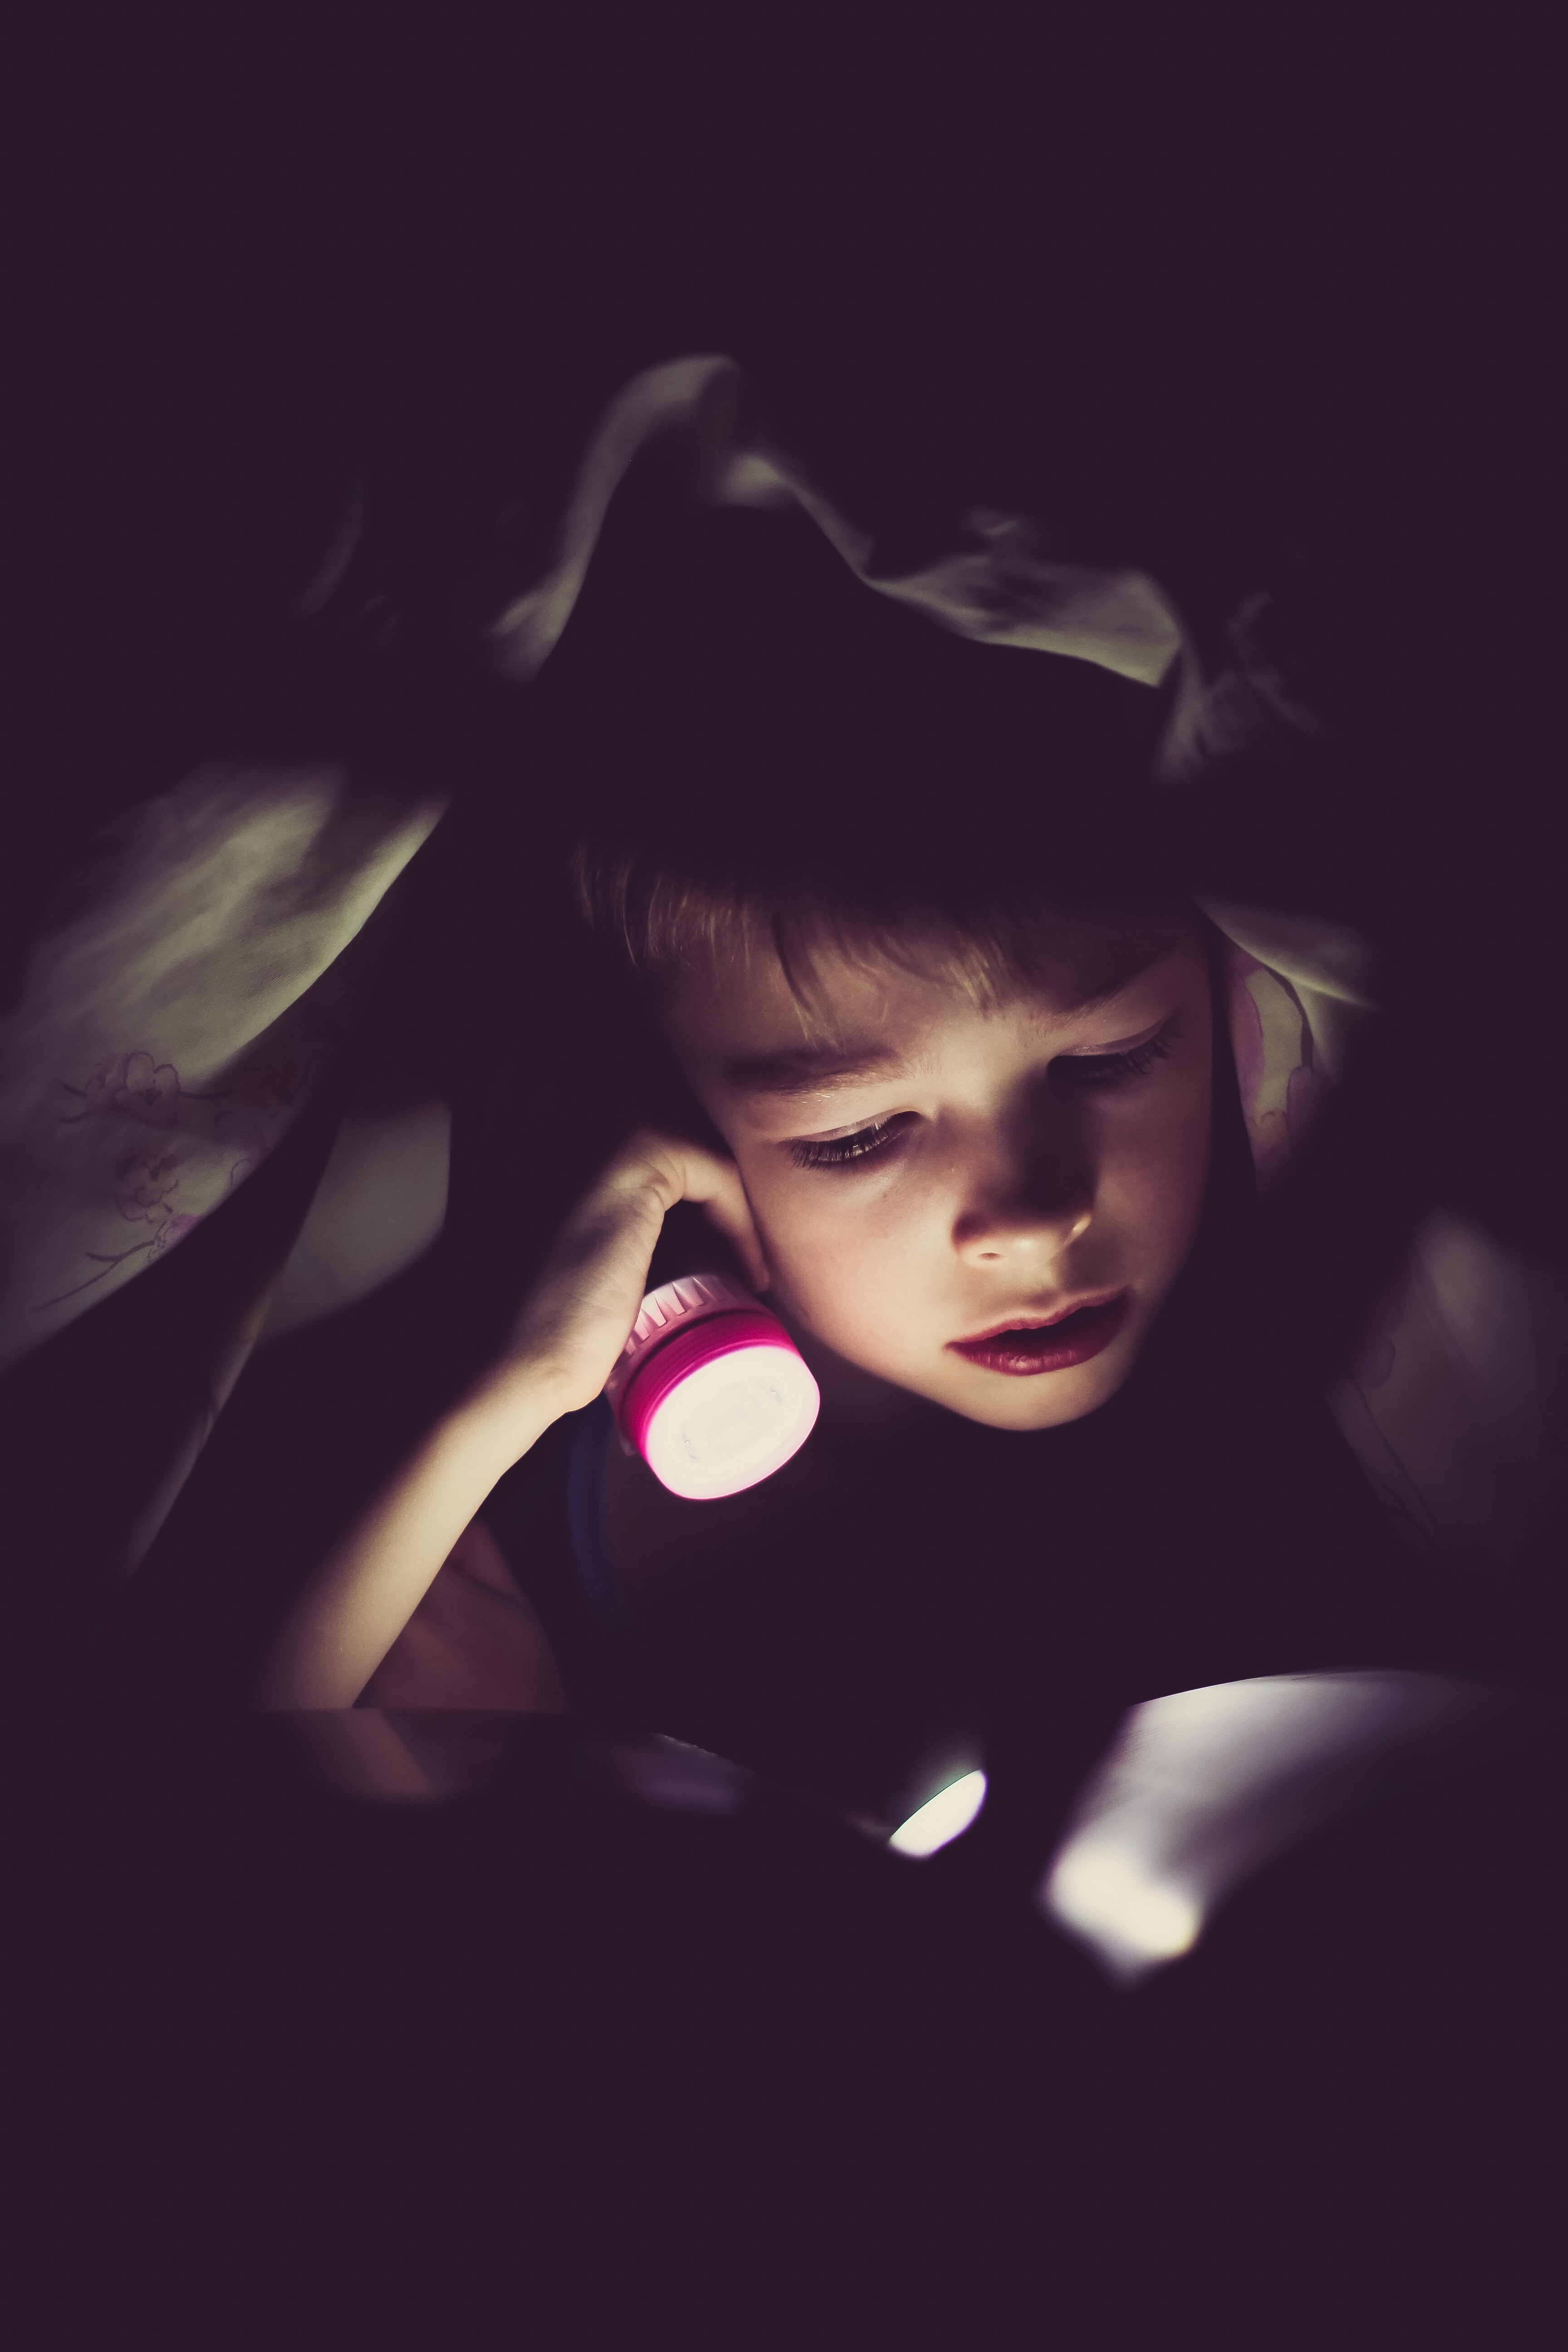
\includegraphics[height=65mm]{story.jpg}
    \source{https://unsplash.com/photos/UYNH5VCsYPU}{https://unsplash.com}
\end{minipage}

\end{frame}
% -----------------------

\begin{frame}
\frametitle{\textbf{The story}}

\begin{displayquote}
    ``I want to have a meetup platform. An adult can create a draft of a meetup and save it. 
    I want to know when the draft has been saved and author's name as well.
    Draft could be published by a publisher. We can only publish a meetup in the time in Future.
    I want to know who publish a draft. When the meetup starts I became a live meetup. 
    When the live meetup ends it became a archived one. \\
    Every meetup has to have title with max. 100 characters and agenda with max. 255 characters.
    \vskip 2mm
    \source{}{The owner}
\end{displayquote}

\end{frame}
% -----------------------

\begin{frame}
\frametitle{\textbf{Think about the solution}}


\includegraphics[height=.8\textheight]{dobromir.jpg}

\end{frame}
% -----------------------

\begin{frame}[fragile]
\frametitle{\textbf{Database first}}

\begin{lstlisting}[language=SQL]
    CREATE TABLE meetups (
        id INT IDENTITY(1,1) PRIMARY KEY,
        status INT NOT NULL,
        title VARCHAR(100) NOT NULL,
        agenda VARCHAR(255) NOT NULL,
        author_name VARCHAR(255) NOT NULL,
        create_at DATE NOT NULL,
        publish_author VARCHAR(255),
        start_date DATE,
        end_date DATE
    );
\end{lstlisting}

\end{frame}
% -----------------------

\begin{frame}[fragile]
\frametitle{\textbf{Code second}}

\begin{lstlisting}[language=Java]
    public class Meetup
    {
        public int Id { get; set; }
        public MeetupStatus Status { get; set; }
        public string Title { get; set; }
        public string Agenda { get; set; }
        public string AuthorName { get; set; }
        public DateTime CreatedAt { get; set; }
        public string PublishAuthor { get; set; }
        public DateTime StartDate { get; set; }
        public DateTime EndDate { get; set; }
    }

    public enum MeetupStatus
    {
        Draft = 1,
        Published = 2,
        Live = 3,
        Archived = 4
    }
\end{lstlisting}

\end{frame}
% -----------------------

\begin{frame}
\frametitle{\textbf{The basics}}

\begin{minipage}{0.45\textwidth}
\begin{center}
    {\fontsize{50}{60}\selectfont \textbf{The basics}}
\end{center}
\end{minipage}
\begin{minipage}{0.45\textwidth}
    \hspace{15mm}
    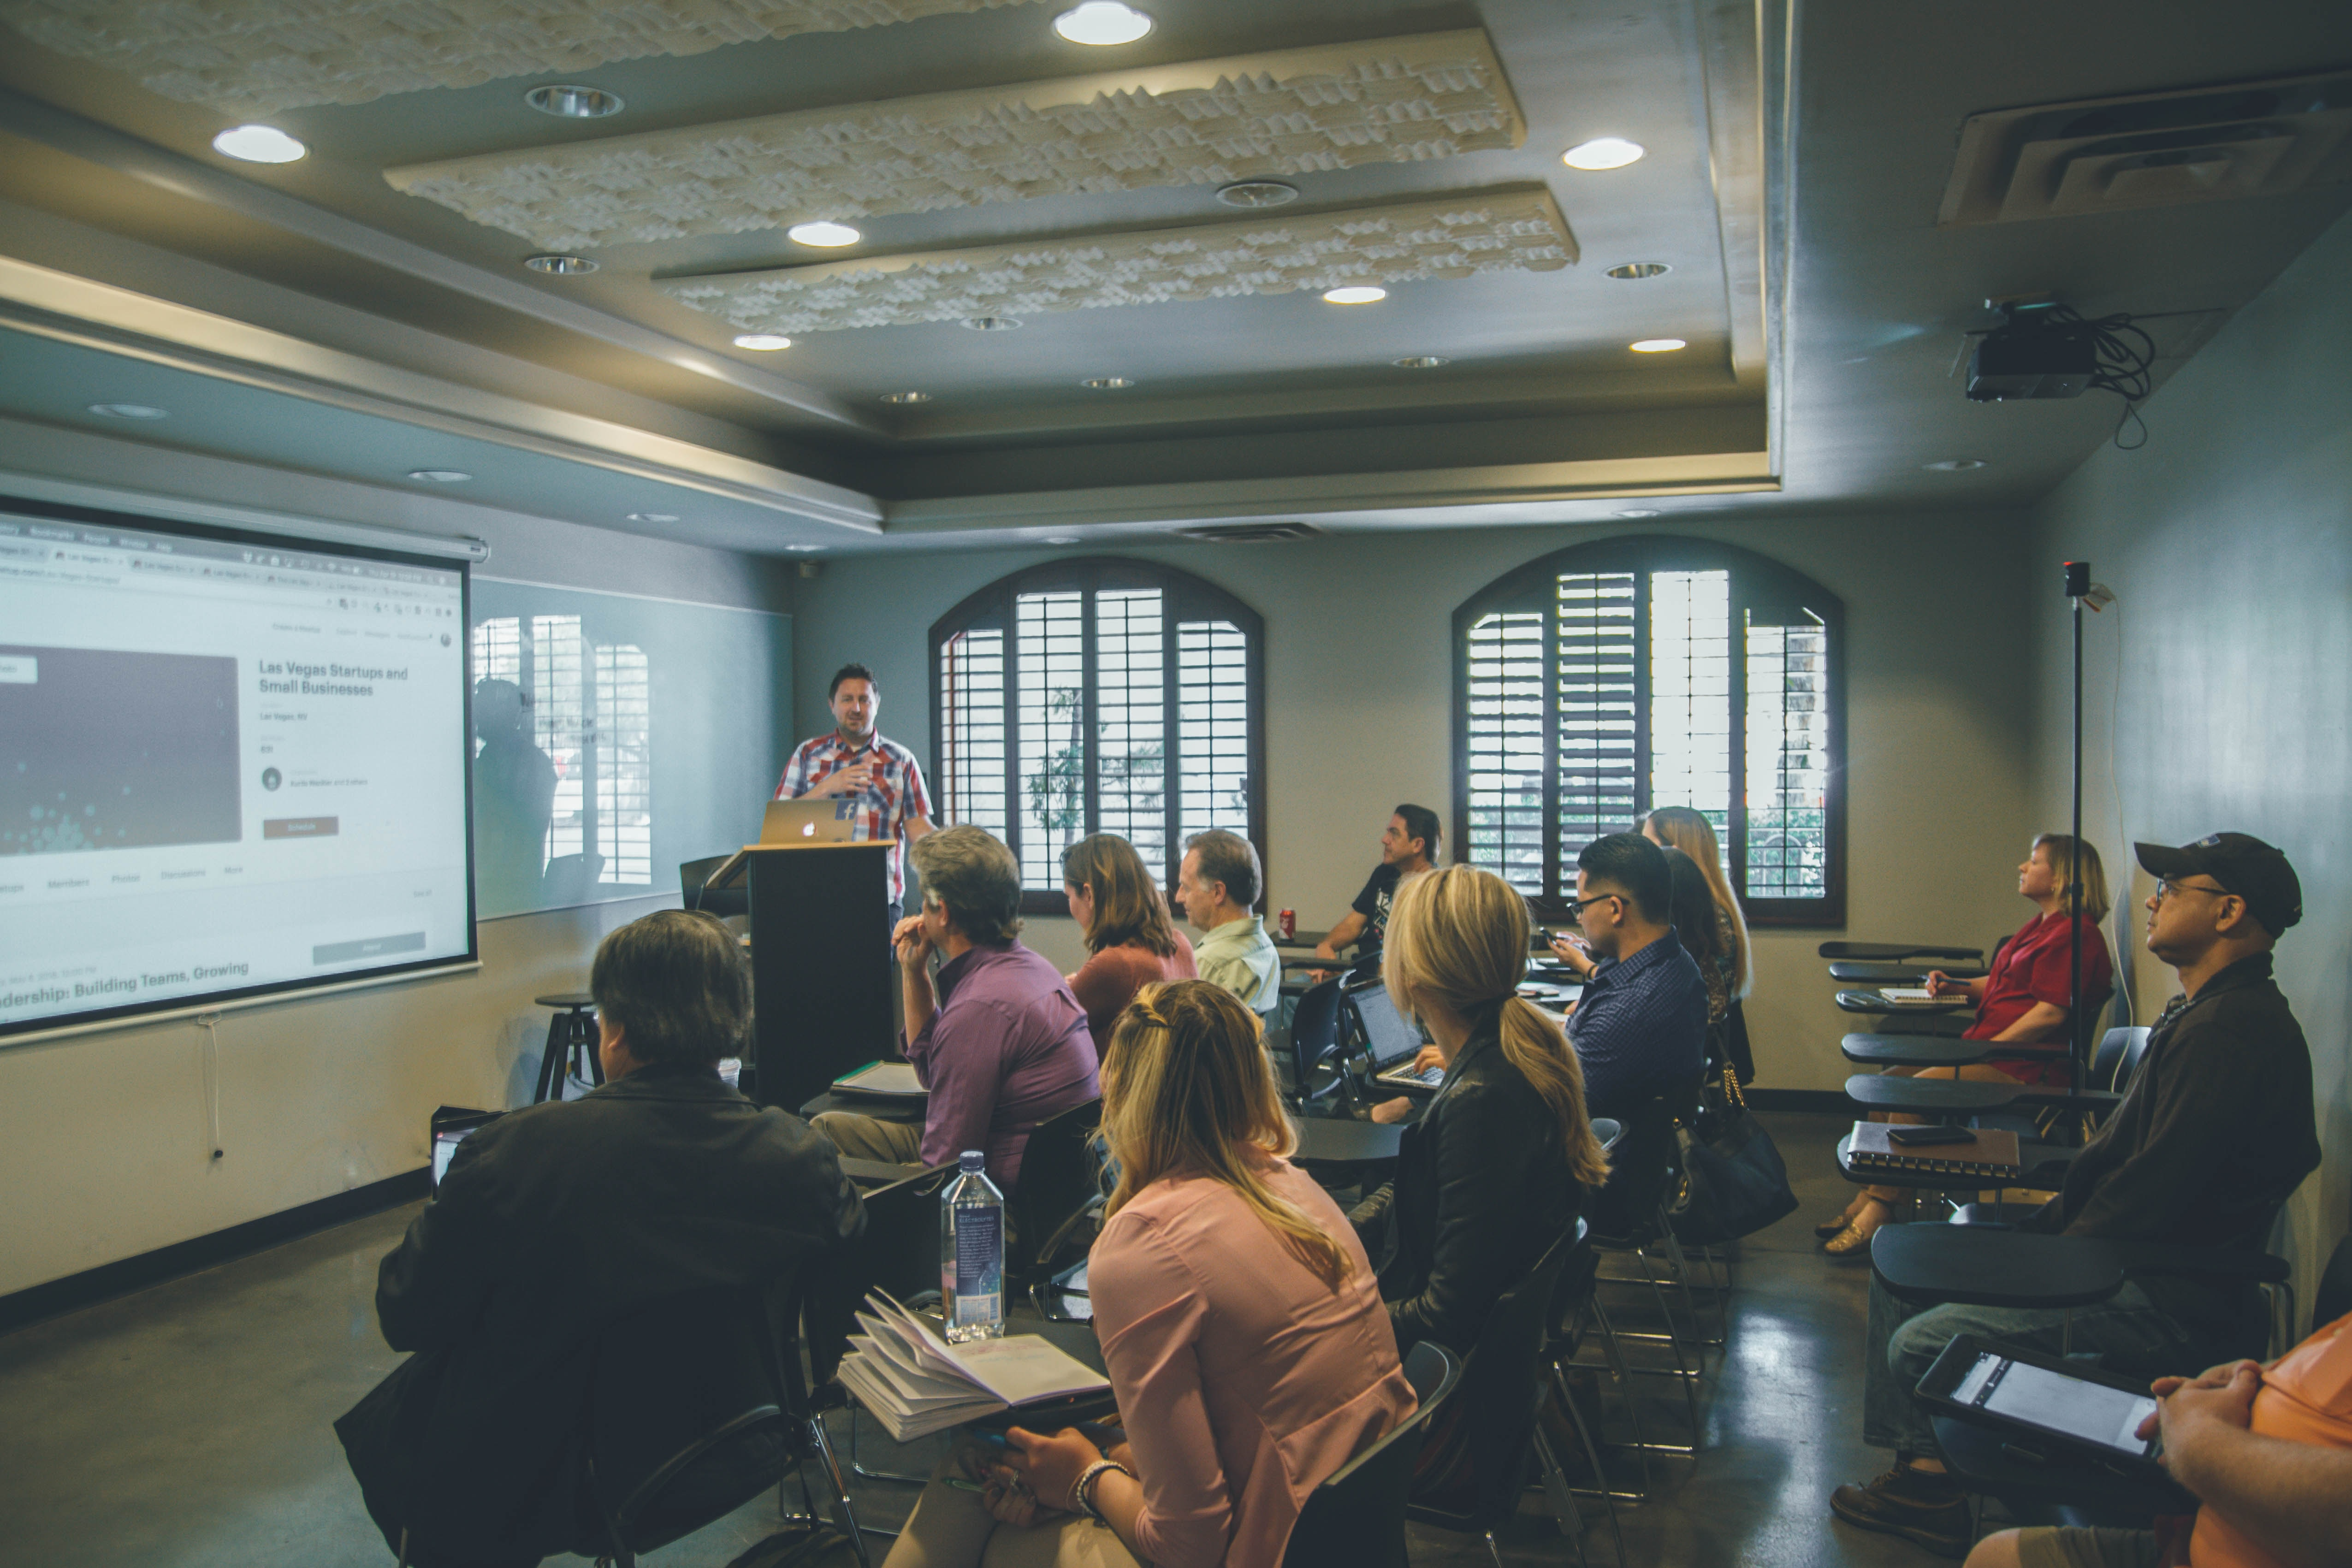
\includegraphics[width=80mm]{basics.jpg}
    \source{https://unsplash.com/photos/1-aA2Fadydc}{https://unsplash.com}
\end{minipage}

\end{frame}
% -----------------------

\begin{frame}
\frametitle{\textbf{Definition}}

\begin{displayquote}
    ``Domain-driven design (DDD) is an approach to developing software for complex needs by deeply connecting the implementation to an evolving model of the core business concepts.``
\end{displayquote}
\vskip 2mm
\source{https://dddcommunity.org/learning-ddd/what_is_ddd/}{dddcommunity.org}


% DDD premise is:
% \begin{itemize}
%     \item Place the project’s primary focus on the core domain and domain logic
%     \item Base complex designs on a model
%     \item Initiate a creative collaboration between technical and domain experts to iteratively cut ever closer to the conceptual heart of the problem.
% \end{itemize}

\end{frame}

% -----------------------

\begin{frame}
\frametitle{\textbf{Building blocks}}

\begin{minipage}{0.4\textwidth}
\begin{center}
    \begin{itemize}
        \item Domain
        \item Ubiquitous language
        \item Bounded Context
        \item Entity
        \item Value object
        \item Invariant
        \item Repository
    \end{itemize}	
\end{center}
\end{minipage}
\hspace{5mm}
\begin{minipage}{0.4\textwidth}
    \begin{itemize}
        \item Factories
        \item Policies
        \item Aggregate
        \item Aggregate root
        \item Services
        \item Domain Event
        \item Command
        \item Query
        \item Exception
    \end{itemize}	
\end{minipage}

\end{frame}

% -----------------------

\begin{frame}
\frametitle{\textbf{Building blocks}}
    
\begin{minipage}{0.4\textwidth}
\begin{center}
    
    \begin{shaded}
        \begin{itemize}
            \item Domain 
            \item Ubiquitous language
            \item Bounded Context
            \item Entity
            \item Value object
            \item Invariant
            \item Repository
        \end{itemize}
    \end{shaded}
\end{center}
\end{minipage}
\hspace{5mm}
\begin{minipage}{0.4\textwidth}
    \begin{itemize}
        \item Factories
        \item Policies
        \item Aggregate
        \item Aggregate root
        \item Services
        \item Domain Event
        \item Command
        \item Query
        \item Exception
    \end{itemize}	
\end{minipage}

\end{frame}

% -----------------------

\begin{frame}
\frametitle{\textbf{Lets code}}

\begin{minipage}{0.45\textwidth}
\begin{center}
    {\fontsize{50}{60}\selectfont \textbf{Lets code}}
\end{center}
\end{minipage}
\begin{minipage}{0.45\textwidth}
    \hspace{15mm}
    
\includegraphics[width=80mm]{code.jpg}
    \source{https://unsplash.com/photos/npxXWgQ33ZQ}{https://unsplash.com}
\end{minipage}

\end{frame}
% -----------------------

\begin{frame}
\frametitle{}

\includegraphics[width=100mm]{Thanks.jpg}
\source{https://unsplash.com/photos/VyC0YSFRDTU}{https://unsplash.com}

\end{frame}
% -----------------------

\end{document}